\section{Organisation du projet}
\label{sec:organisation}
    Le projet s’organise en deux phases distinctes. D'abord, la phase d’analyse et de conception, qui consiste
    à analyser les besoins et les objectifs du projet (ce afin de faire un choix sur les technologies
    sélectionnées pour la réalisation de l’application), au découpage des tâches principales qui seront
    réalisées par la suite, et à la réalisation de l’architecture principale avec la base de données envisagée
    et les différentes parties de la plateforme web. On sera amené à effectuer des tests pour voir ce qu’il
    est possible de faire avec la technologie envisagée, et on réalisera aussi une ébauche qui permettra
    d’avancer plus rapidement par la suite.

    Cette phase donnera lieu à 3 rapports. Ce rapport de pré-étude décrit le contexte du projet,
    l’étude de l’art et une analyse des solutions possibles. On rédigera ensuite un rapport de spécifications fonctionnelles
    qui détaillera la solution envisagée, les fonctionnalités détaillées de la plateforme et l’architecture
    de celle-ci, puis enfin le document de planification initial qui détaillera le calendrier des tâches et
    l’ordonnancement de celles-ci. Deux soutenances auront lieu suite à cette phase ; la première pour présenter
    le projet et la seconde pour présenter la planification initiale du développement de la plateforme.

    La phase de réalisation, elle, consiste au développement de la plateforme à proprement parler.

    \subsection{Calendrier de la phase d’analyse/conception}
    \label{subsec:calendrier}

    \begin{figure}[ht!]
        \centering
        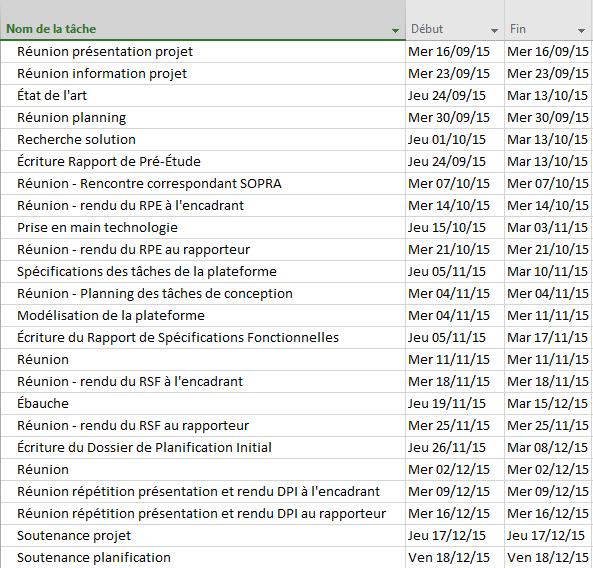
\includegraphics[width=1\textwidth]{figure/planning_description.png}
        \caption{Liste descriptive des tâches du planning d'analyse}
        \label{fig:description}
    \end{figure}

    \begin{figure}[ht!]
        \centering
        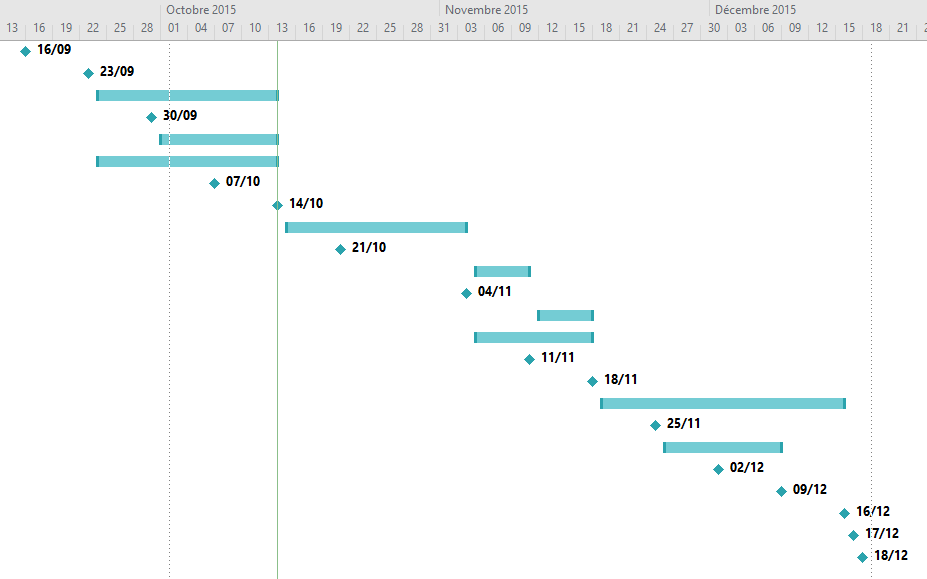
\includegraphics[width=1\textwidth]{figure/planning_schema.png}
        \caption{Schéma du planning d'analyse}
        \label{fig:schema}
    \end{figure}


